\section{Problema e público-alvo}

Há uma grande gama de dados metereológicos no estado de São Paulo, mas eles estão espalhados em diferentes orgãos públicos: INMET, CEMADEN ou em estações privadas como a estação metereológica presente no ICTS, parte do smartcampus. Além disso, não se sabe quais estações possuem dados confiáveis.
\par O objetivo do ClimaSP é utilizar um sistema de agregação de várias estações e utilizar algoritimos para indicar o indice de confiaça desses dados para uma certa região de São Paulo.
\par Este projeto tem como público alvo:
\begin{itemize}
    \item \textbf{cientistas:} pois, como é um agregador com nível de confiança, seus preprocessados pódem ser utilizados para o treinamento de IA e outros estudos.
\end{itemize}

\begin{figure}
    \centering
    \begin{subfigure}{0.48\linewidth}
        \centering
        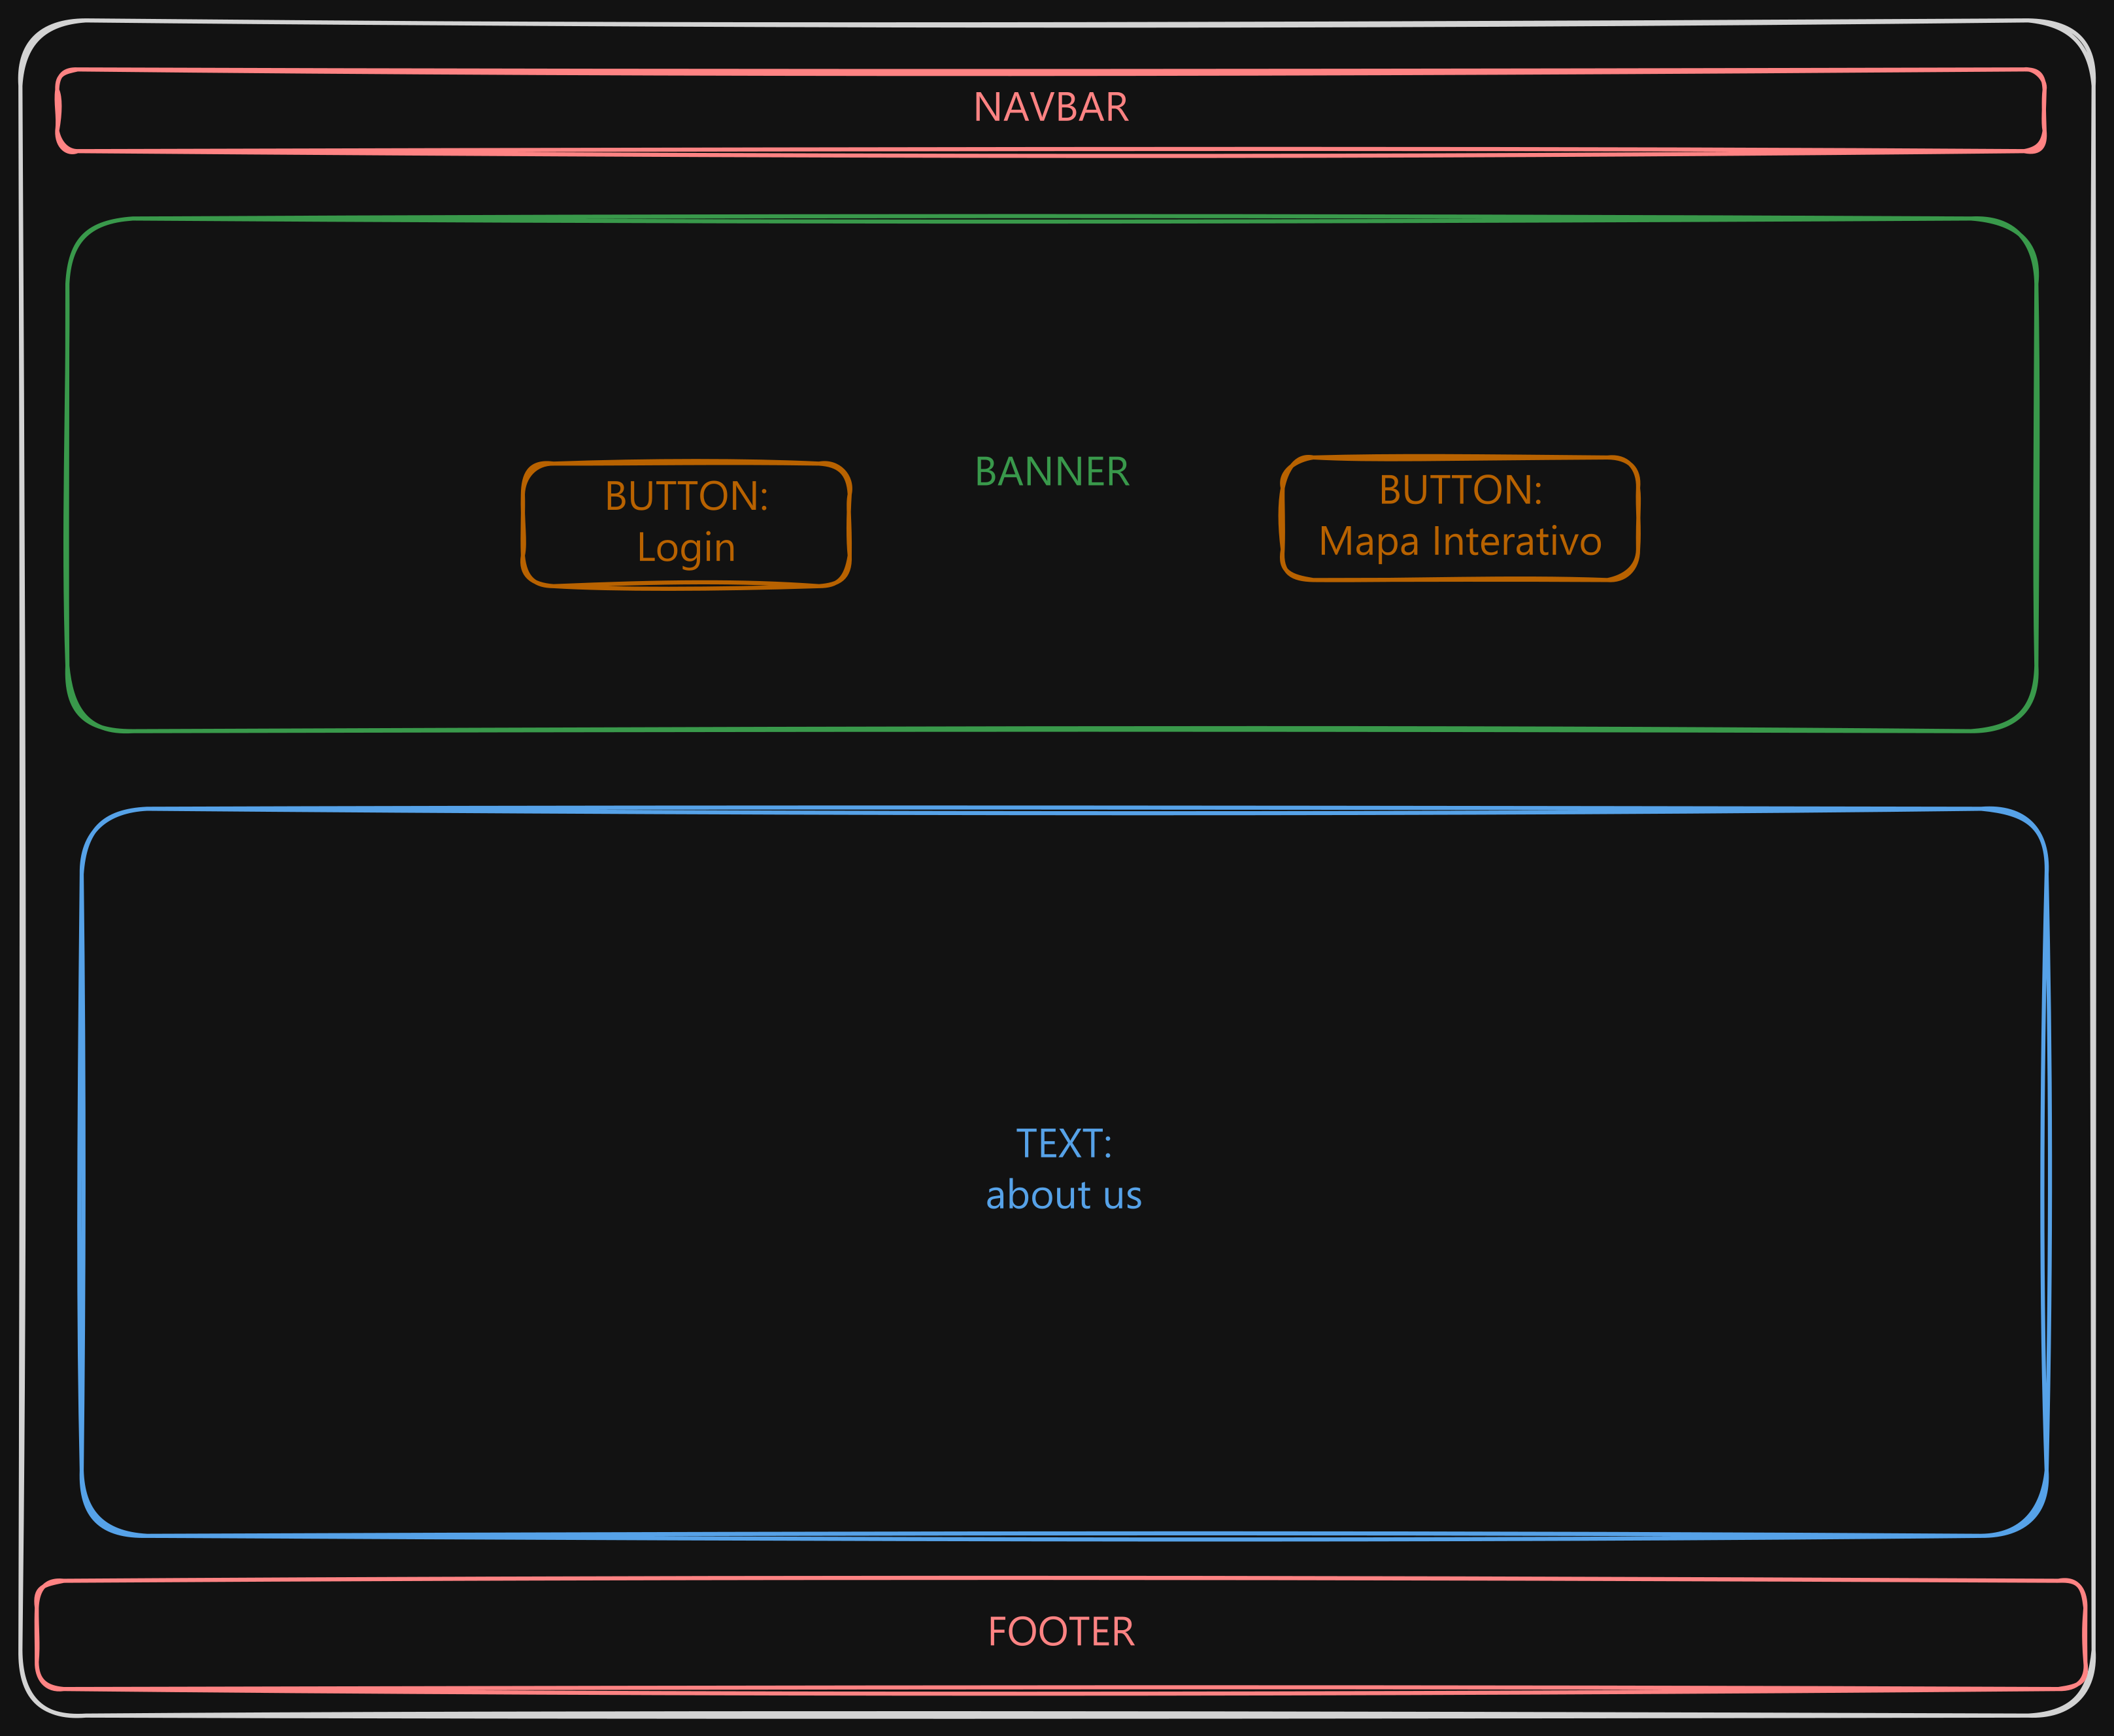
\includegraphics[width=\linewidth]{../imagens/site-home.png}
        \caption{Página inicial}
    \end{subfigure}
    \hfill
    \begin{subfigure}{0.48\linewidth}
        \centering
        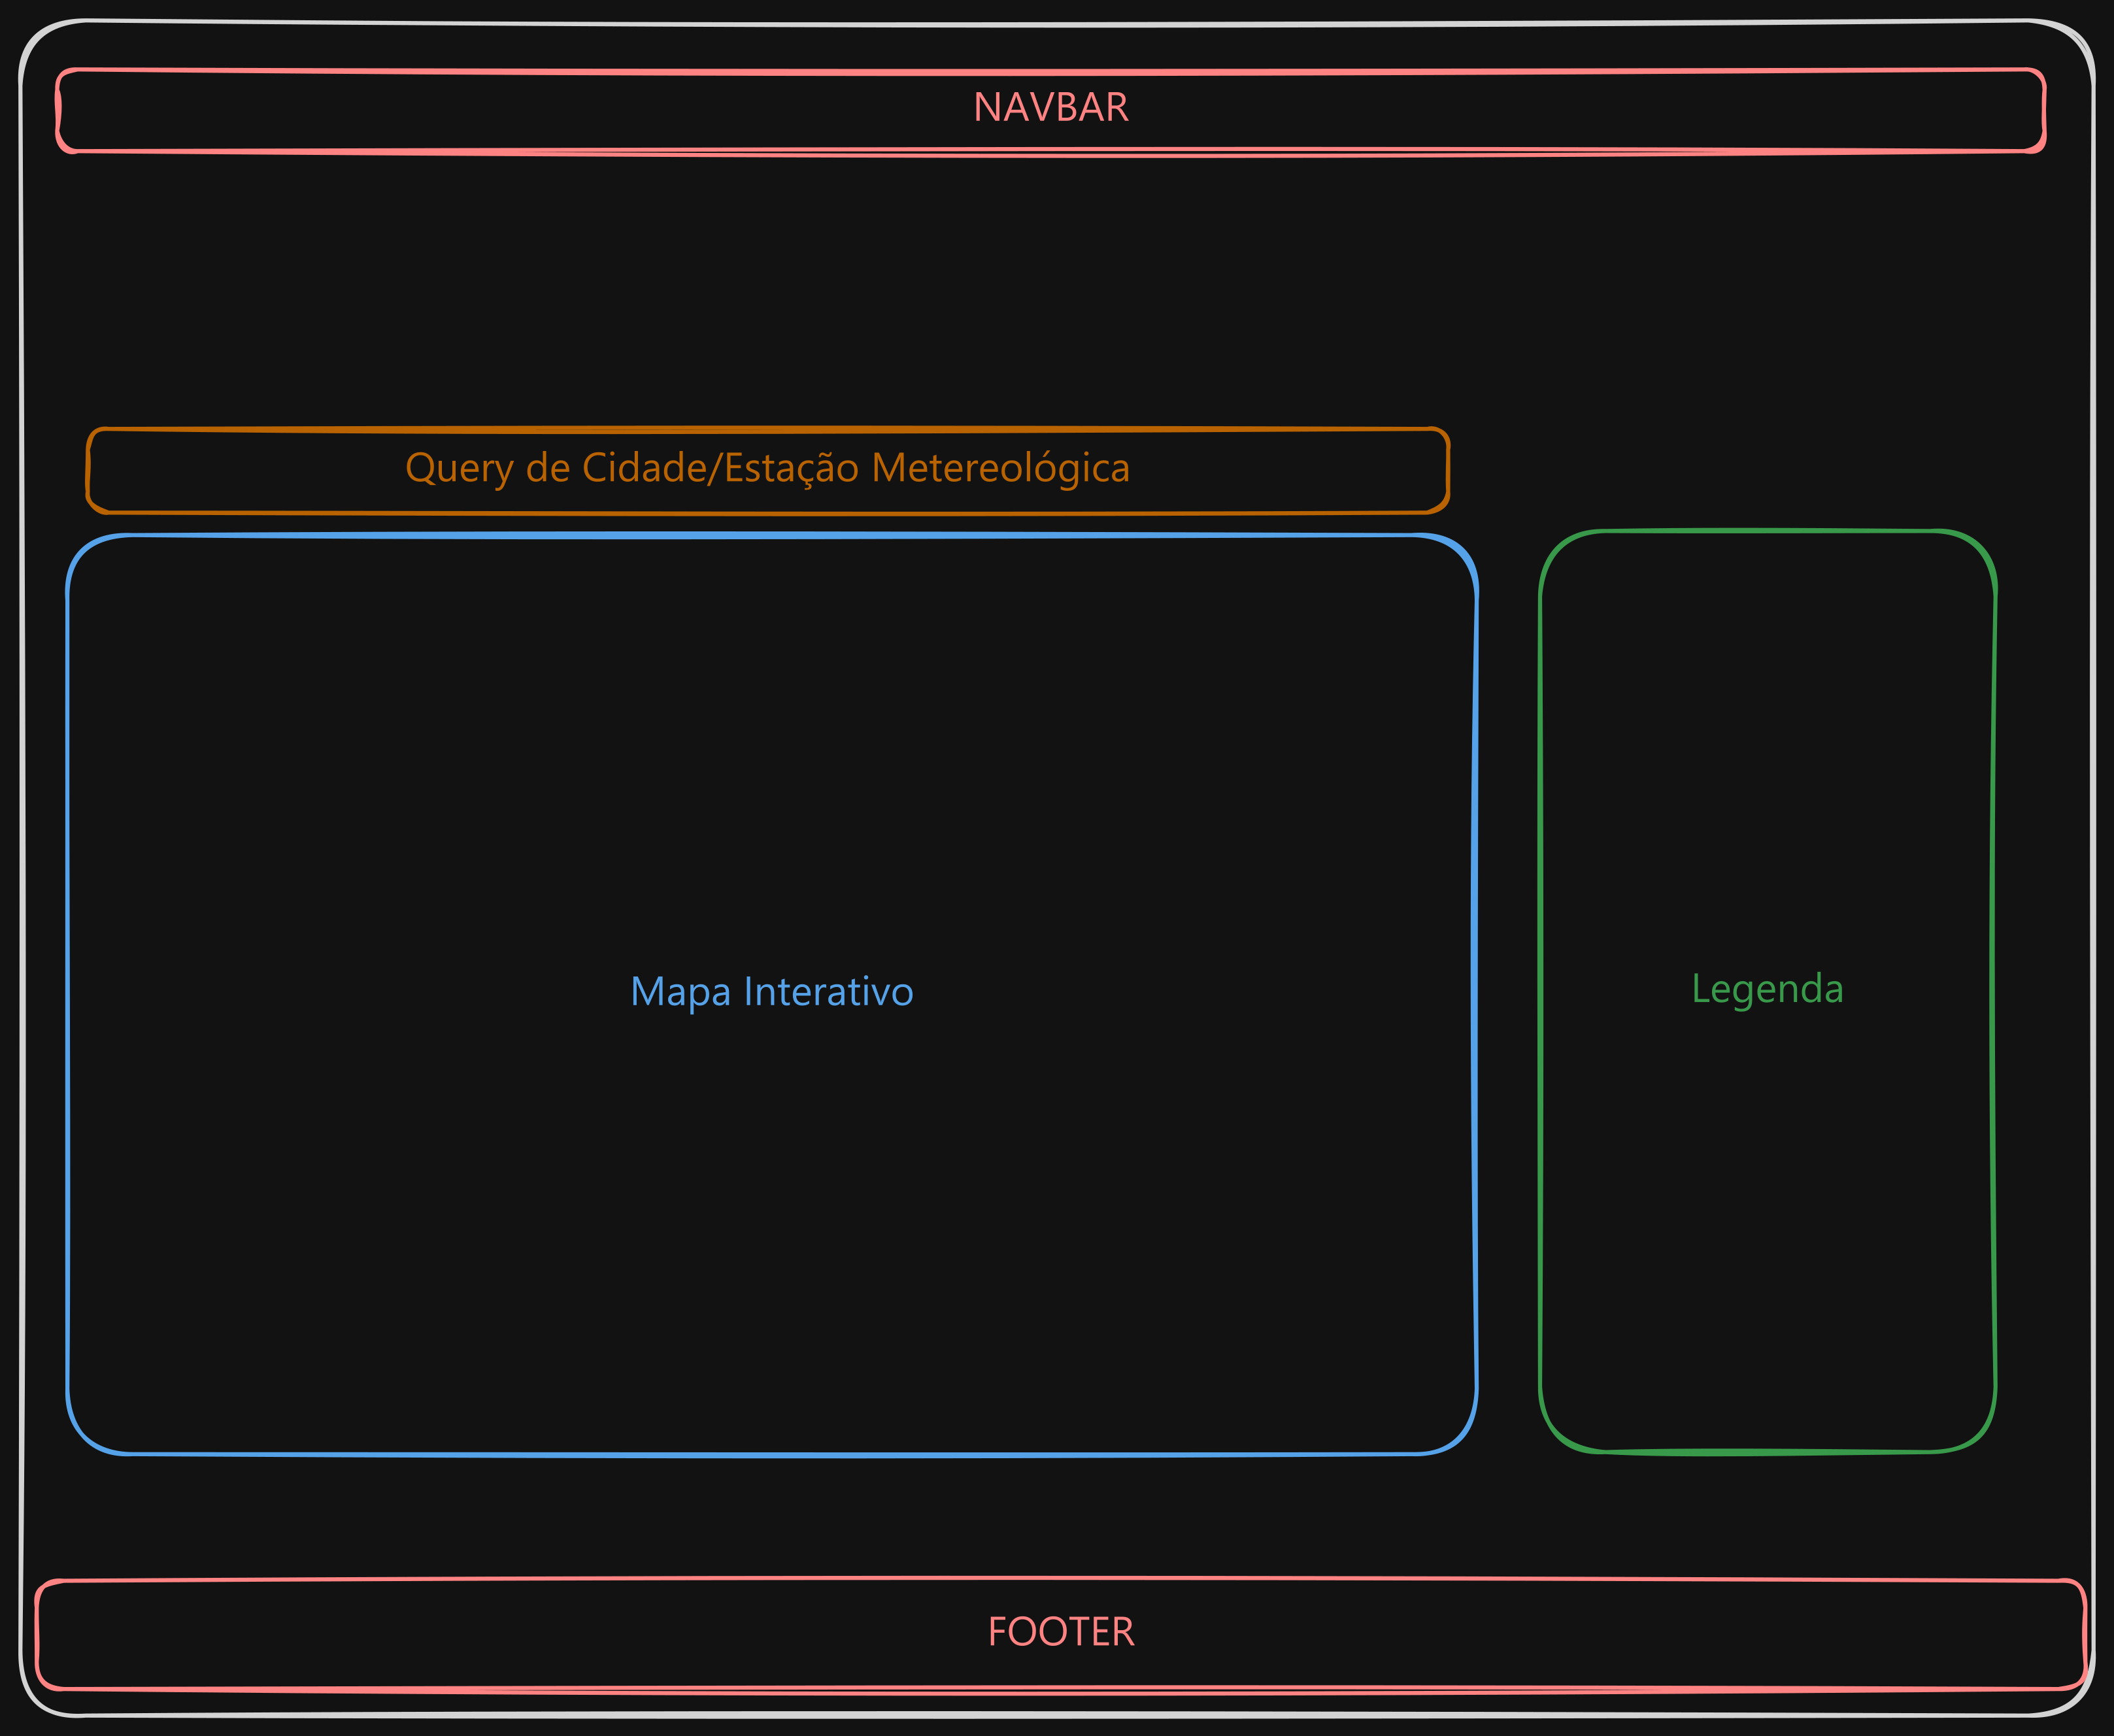
\includegraphics[width=\linewidth]{../imagens/site-mapa.png}
        \caption{Mapa interativo}
    \end{subfigure}
    
\end{figure}
